\usetikzlibrary{arrows.meta,automata,positioning}
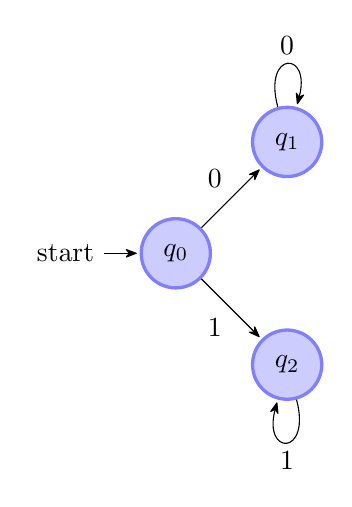
\begin{tikzpicture}[shorten >=1pt,node distance=2cm,on grid,auto,
  >={Stealth[round]},
  every state/.style={draw=blue!50,very thick,fill=blue!20}]
\node[state,initial] (q_0) {$q_0$};
\node[state] (q_1) [above right=of q_0] {$q_1$};
\node[state] (q_2) [below right=of q_0] {$q_2$};
\path[->] (q_0) edge node [above left] {0} (q_1)
   edge node [below left] {1} (q_2)
   (q_1) edge [loop above] node {0} ()
   (q_2) edge [loop below] node {1} ();
\end{tikzpicture}
